\section{Method} \label{sec:method}

In this section, the researched method itself is explained.
Before describing important steps in the method in detail, we give an overview over the method.
The first step is to take a classified graph dataset (training set), and subjected all graphs to the WL-labeling scheme up to a specified fixed number of iterations (algorithm \ref{alg:WLlabeling}).
During this, the corresponding WLLT is constructed (algorithm \ref{alg:WLLTconstruction}).
After the complete construction of the WLLT, it is equipped with initial edge weights (section \ref{subsec:WLLT_ew_init}).
This allows to define vector representations of the graphs (section \ref{subsec:graph_representation}).
Now machine learning is applied, to iteratively update these edge weights (section \ref{subsec:EWL}).
The update decision is based on decreasing the distance between graph samples from the same class, and increasing the distance between sample from different classes.
It is crucial to notice, that changing the distance between two samples influences edge weights in the WLLT, which may be used to compute the distance between many other samples.
The performance of the learner is instead measured on the resulting distance matrix for all graphs.
Some of the used performance evaluation is presented at the end of this section, too.

\subsection{Graph Representation} \label{subsec:graph_representation}

	One of the easiest data-structures to represent complex structure data are fixed-size vectorial representations.
	Similarly to the approach used in the No-graph kernel proposed by \citeauthor{2021_Schulz_CONF}, we used a vertex label histogram as graph representations.
	However unlike the histogram used for the definition of the No-graph kernel, the vertex labels we use, compress information on the structure of the (labeled) graph.
	We define the \textbf{graph representation} (graph \textbf{feature vectors}) $r_G$ for a graph $G$ in the following way.
	Let $T$ be the WLLT with $p$ vertices ($|V(T)|=p$) and depth $D$ (i.e., $D$ iterations of WL-labelings were performed on the graph dataset).
	Note, that this includes an artificial root and $p-1$ assigned WL-labels, where the WL-labels of the zeroth iteration are the original vertex labels in the graph dataset.
	Further note, that all labels in the WLLT are distinct.	
	For a graph $G$ let $S_i$ denote the set of vertices, that were assigned the label $i$ in any of all $D$ iterations of the labeling scheme:
	\[ S_i := \{ v\in V(G)| \exists j:\ \ell_j(v)=i \} \]	
	Now define the graph representation $r_G$ of $G$ as the normalized distribution of WL-labels among the vertices of $G$:
	\begin{equation} \label{eq:graphrepr}
		r_G := \frac{1}{|V(G)|} \big( |S_0|, |S_1| \dots |S_p| \big)\ \in\IR^{p}
	\end{equation}
	For high $D$ and a diverse dataset (implying a high value of $p$), it is expected that these representations are sparse vectors.
	
\subsection{WLLT Edge Weight Initialization} \label{subsec:WLLT_ew_init}
	
	Since we measure the performance of the learner by comparison to the initial state (recall section \ref{subsec:research_question}), the initialization of the edge weights in the WLLT effect the computations and evaluations significantly.
	The edge weights are used additatively in the computation of the distance between two vertices (WL-labels) in the WLLT (recall the definition of \textbf{distance} in section \ref{subsec:def_graphtheory}). 
	Furthermore, we require non-negative edge weights for a resulting positive definite Tree-sliced Wasserstein Kernel (section \ref{subsec:def_WassDist}).
	Thus it is reasonable to initialize the edge weights with positive values.
	In all edge weights in the zeroth layer of the WLLT, that is the weights of all edges incident to the root, completely define the distances between the zeroth WL-labels.
	If initial vertex labels are known and used as zeroth WL-labels, one may use application based knowledge to initialize these edge weights.
	Otherwise, and for all other edge weights, the uniform initialization is reasonable.
	This way, the tree-structure itself ensures that WL-labels of different subtrees are further apart, which reflects the idea of the WL-labeling scheme.
	For most experiments and during the development of the method, a uniform initialization to value $1.0$ (with no prior application based knowledge) was used.
	
	Other possible initialization, like based on a gradient through the depth of the WLLT (fixed or based on the layer size) may be applicable too.
	One may assume that the learning process could be able to reach a desirable configuration, largely independently of the initialization.
	The experiments however were not extensive enough do not support this assumption empirically.

\subsection{Edge Weight Learner} \label{subsec:EWL}
	
%	For reference, the processes described in this subsection are implemented in the script \texttt{x3\_wllt\_edge\_weight\_learner.py}.	
	In order for the edge weight learning to begin, a complete WLLT (up to some depth and with edge weights), the feature vectors (section \ref{subsec:graph_representation}) of all graphs, and the graph classifications must be given.
	The outer loop in the computations performed by the edge weight learner, loops over all learning epochs and returns newly defined edge weights each time.
	Each learning epoch consists of an inner loop over the graph samples in a chosen batch of graph samples for this learning epoch.
	Since the inner loop loops over all pairs of graphs (computing their distance), the batch size enters quadratically into the calculation of the runtime of the learning process.
	Before starting the first epoch, the batches for every epoch are constructed.
	To simplify later computations, each such batch contains approximately the same number of graphs from every given class.
	If the sizes of different graph classes vary greatly, this is not ideal, with respect to an equalized weighting of the graph samples. 
	To diminish such issues, the batch sizes were chosen accordingly for the respective datasets.
	For each learning epoch, all different graph combinations of the graphs in the batch are used to compute a  weight update $\Delta w$ for the WLLT edge weights $w$:
	\[ w^\prime = w + \eta * \Delta w \]
	Here, $\eta\in(0,1]$ is the learning rate.
	Let $r_{G_0}, r_{G_1}\in\IR^p$ be the graph representations for two graphs and $w\in\IR^p$ the vector of current edge weights in the WLLT.
	Recall equation \ref{eq:TreeWassDist} with distributions $\mu = r_{G_0}$ and $\nu=r_{G_1}$.	
	Denote the weighted difference vector between the graphs as $\Delta r_{G_0, G_1} \in\IR_+$:
	\[ \IW_{d_T}( r_{G_0}, r_{G_1} ) = \sum_{e\in E} \underbrace{ w(e) \ \Big| r_{G_0} \big( \Gamma(e_c) \big) -  r_{G_1} \big( \Gamma(e_c) \big) \Big| }_{=: \Delta r_{G_0, G_1}(e)} = \sum \Delta r_{G_0, G_1} \]
	
	Now if the graphs are in the same class ($c(G_0) = c(G_1)$), their distance $\IW_{d_T}( r_{G_0}, r_{G_1} )$ shall be decreased, and increased otherwise.
	To effect as little other distances as possible, we update only the edge weights $w(e)$ where $\Delta r_{G_0, G_1}(e) \neq 0$.
	These are exactly all edge weights, which contribute in the computation of the Wasserstein distance between the considered graphs.
	Let $\delta^>$ be an indicator function such that $\delta^>(x)=\{i| x_i>0 \}$.
	If not stated otherwise, in the following we simplify the notation by writing ${w}_{\delta^>(\Delta r_{G_0, G_1})}$ as $w$.
	We use a \textbf{pull factor} $f_{\text{pull}}\in(0,1]$ and a \textbf{push factor} respectively $f_{\text{push}} \in(0,1]$ and set:
	\begin{equation} \label{eq:DeltaW}
		\Delta w = \begin{cases}
			f_{\text{pull}} w &\text{if } c(G_0) = c(G_1)\\
			f_{\text{push}} w &\text{otherwise}\\
		\end{cases}
	\end{equation}
	Notice that by definition of the push and pull factors (\textbf{pp-factors}), and the learning rate, the edge weight update is the addition or subtraction of a fraction of the already used weights.
	Thus the weights remain non-negative during all learning epochs.
	As mentioned, this is desired in order to use the resulting tree metric in the definition of a graph kernel.
	
	If the edge weights were updated after each sample, the order of sample from the same class and from different classes would matter and the batch size has effectively size one.
	To prevent this, all weight updates during one learning epoch are stored but not applied.
	Applying all updates afterwards may lead to an exponential scaling effect, which we naturally would like to avoid.
	Thus, after each epoch the mean of all computed (non-negative) updates is applied.
	
	Using the Wasserstein distance here to align the structural graph representations may be beneficial in capturing more complex characteristics of the graph, compared to taking the mean or other additive simplifications as were used for the definition of many graph convolution kernels (see related work in section \ref{subsec:related_work})~\cite{2019_Togninalli_NIPS}.
	
	\paragraph{Absolute pp-Factors}
	The described edge weight update has the benefit, that the edge weights remain non-negative all the time.
	However the definition of the weight delta as a percentage of existing weight may seem unusual.
	To compare the effects of a more traditional, additive update, such an update was implemented too.
	Using this setting in the learner, uses the following definition: 
	\begin{equation}\label{eq:DeltaW_Abs_pp_factors}
		\Delta w = \begin{cases}
			f_{\text{pull}} &\text{if } c(G_0) = c(G_1)\\
			f_{\text{push}} &\text{otherwise}\\
		\end{cases} 
	\end{equation}
	
	Since we do not need to fear exponentially de- or increasing weights in this setting, the accumulated weight updates are applied after each epoch without taking their mean.
	
	\paragraph{Class-Imbalance Factor}
	Since the update mechanism increases the edge weights for graphs from different classes and decreases the edge weights graphs from the same class, 
	depending on the number of classes and their sizes, the relation between added and removed weight may vary greatly.
	To ensure better comparability between datasets, and for example different fractions of dataset, we reduce this effect by introducing a factor which we refer to as \textbf{class imbalance factor}.
	
	Let $m$ be the batch size, and let there be $n$ (selected) graphs for every of $c$ classes in each batch.
	The number of possibilities to draw two graphs from the same class $p_S$ amounts to the number of possibilities to draw the first graph from one fixed class ($n/2$), times the number of possibilities to draw
	a second, different graph from the same class ($(n-1)/2$).
	One may summarize these possibilities to $n\choose2$ as well.
	This has to be calculated for every of the $c$ classes.
	Thus it is:
	\[ p_S = {n \choose 2} c = \frac{n(n-1)}{2} c \]
	The number of possibilities to draw two graphs from different classes $p_D$ amounts to the number of possibilities to draw two graphs, each from two different fixed classes ($nn$), times the number of possibilities to draw
	such two different classes (${c \choose 2}$).
	Thus it is:
	\[ p_D = nn{c \choose 2} = \frac{cnn(c-1)}{2} \]
	Since these factors are used only for scaling the applied weights, we ignore the common factor $nc/2$.
	Now one can scale the weight update of same class samples with $1/n-1$ and different class samples with $1/n(c-1)$.
	This however greatly decreases the weights, and in the implementation these factors were scaled, such that only different class samples are scaled by $1 / ((n-1)n(c-1))$.
	Thus the mentioned push factor in equations \ref{eq:DeltaW} and \ref{eq:DeltaW_Abs_pp_factors} is scaled accordingly: 
	\[f_{\text{push}} = \frac{ f_{\text{push}} }{ (n-1)n(c-1) }\]
	
	\paragraph{Weights Scaling}
	Using the absolute pp-factors requires to prevent negative edge weights, which where set to zero. 
	On top of that the first experimentation showed, that the multiplicative weight update (according equation \ref{eq:DeltaW}) has the potential to define exponentially increasing edge weights and thereby skewing the overall used edge weight vector.
	To prevent this effect, a parameter setting allows to set an upper bound for the weights too.
	The standard setting is $[0,2]$, which is as powerful as scaling to the uniform interval $1.0$, but more suitable to the described intuitive uniform edge weight initialization to the value $1.0$ as the mean of the tolerated interval (section \ref{subsec:WLLT_ew_init}).
	
	\paragraph{Heaviest Earth Threshold}
	The method described so far updates all edge weights in the subtree of the WLLT that includes the root and all leaves, associated with positive entries in $\Delta r_{G_0, G_1}$ for two graphs $G_0$ and $G_1$.
	And the strength of the updates may depend on the pp-factors (the classes of the graphs), the number of graph classes and their sizes and may be limited to an interval.
	
	Now consider the following example.
	Let $G_0$ and $G_1$ bet two almost identical graphs of the same class, but $G_1$ contains one vertex more, with an WL-label, which does not occur in $G_0$.
	Since the structures of the graphs are almost identical, the method should focus on decreasing the importance of the distinct label (to decrease the distance between the two graphs).
	However, since the graphs do not have the same number of vertices, their graph representations are likely to be different at almost any non-zero position (recall the normalization of the graph representation).
	Thus the so far described update method may decrease the weights to almost all associated WL-labels and impact the distances to other graphs greatly.
	
	To limit the update effect in similar cases, and to reduce the overall introduced or subtracted weight, we define a parameter we call \textbf{Heaviest Earth Threshold} $h$.
	Using the definitions from above, ${w}_{\delta(\Delta r_{G_0, G_1})}$ is the vector used for the computation of the Wasserstein Distance.
	In tribute to the name Earth Mover Distance, this vector can be seen as the costs or weight of the earth which is needed to align the given distributions.
	Thus we can use $h$ to focus the weight update on the WL-labels, which have the most impact to the computation of the Wasserstein distance.
	Let $H$ be the $h$-th highest value in $w$.	
	Using an indicator function $\delta^\ge$ such that $\delta^\ge(x)=\{i| x_i\ge0 \}$, we only the updated weights with the indices
	\[ \delta^+(\Delta r_{G_0, G_1}-H ) \]
	These are all edge weights, which contribute at least the the $h$-th heaviest values to the distance computation.
	Notice, that the usage of the Heaviest Earth Threshold is effectively canceled, if it is set to the dimension of the weight vectors ($h=\dim(w) = p$).
	
	In the implementation and when reporting the experiments in section \ref{subsec:experiments} we refer to Heaviest Earth Threshold as $t_{\text{he}}$.
	This notation gives the percentage of non-zero edge weights which shall be updated.
	$h$ is set accordingly.
		
	\paragraph{Runtime}
	
	As already discussed, the computation of $d$ iterations of WL-labels for a graph with $m$ edges can be done in $\mathcal{O}(dm)$ (section \ref{subsubsec:def_WLlabeling}).
	Notice that constructing a graph representation has runtime $\mathcal{O}(dm)$ too (independently of the existence of the WLLT).
	and the construction of the WLLT for $N$ graphs with at most $m$ edges in $\mathcal{O}(Ndm)$ (section \ref{subsubsec:def_WLLT}).
	Let there be $p$ WL-labels in the WLLT.
	Thus the graph representations have dimension $p$.
	The computation of the distance between two graphs with known graph representation can be done in $\mathcal{O}(p)$ since it requires a subtraction, taking the absolute value and addition of two $p$ dimensional real graph representations.
	Notice that this is a significant improvement over one of the native computation of the Wasserstein Distance (see equation \ref{eq:discreteWassDist}), which has cubic runtime complexity ($\mathcal{O}(n^3 \log(n))$, where $n$ gives the maximum number of vertices)~\cite{2019_Togninalli_NIPS}.\footnote{Although the naive computation can be improved to a near-linear time computation as well, when utilizing some tricks like the Sinkhorn regularisation~\cite{2019_Togninalli_NIPS}.}	
	For two graphs with unknown representation, which both have at most $m$ edges, it requires a runtime in $\mathcal{O}(mh+p)$.
	
	The learning procedure runs linearly in the number of requested learning epochs $e\in\IN$.
	However the runtime of one learning epoch grows quadratically in the batch size $b$ since all different pairs of graphs are used.
	In side the batch loop, the candidate selection step requires to sort a $p$ dimensional real vector, which can be done in $\mathcal{O}(p\log(p))$.
	The other operations inside the batch loop have runtime linear in $p$.
	The other operations outside of the batch loop have runtime linear in $p$ as well (e.g. accumulating and averaging the weight update).
	Thus the learning procedure for $e$ epochs, $b$ graphs per batch and an already constructed WLLT with $p$ vertices and already constructed graph representation vectors has runtime complexity
	\[ \mathcal{O}\big(e(b^2 p\log(p) + p)\big) \]
	
	These theoretical considerations should be supported by runtime measurements on implementations.
	Since the the focus of this thesis lies on the functionality and applicability of the proposed approach, and since the theoretical runtime is comparative to other kernels,
	runtime measurements experiments were omitted.
	
\subsection{l-WWLLT Kernel} \label{subsec:lWWLLTkernel}
	
	In order to apply a multitude of different tools from Machine Learning and to compare the performance of the implemented learner, we would like to translate the computed distance measure into a graph kernel.
	Given the WLLT $T$, and an non-negative edge weight vector $w\in\IR^+$ (learned or defined) on it, we can compute a distance matrix $D$ for any set of graphs $\mathcal{G}$ by using the graph representations defined in equation \ref{eq:graphrepr} and the introduced Tree-slice Wasserstein distance from equation \ref{eq:TreeSlicedWassersteinDistance}:
	\[ D = \Big\{ \IW_{w}( r_{G_0}, r_{G_1} ) \Big\}_{G_0, G_1 \in\mathcal{G}} \]	
	
	We can make use of the Tree-sliced Wasserstein kernel (section \ref{sec:def_TSWKernel}) and set
	\[ k_{\text{lWWKKT}}(G_0, G_1) := \exp\big( -\lambda \IW_{w}( r_{G_0}, r_{G_1}  \big) \]	
	Since this Wasserstein distance is positive-definite (following the argumentation with non-negative edge weights in~\cite{2019_Le_NIPS}),
	the kernel is positive definite as well (following Theorem C.3.2 in \cite{2017_Bollobas_BOOK} and the argumentation in ~\cite{1938_Schoenberg_CONF}).
		
	For the kernel coefficient $\lambda$ a few parameters were used in the experiments.
	By far the best configuration was setting it as the inverse of the number of graphs (dimension of the computed distance matrix)\footnote{In accordance with \textit{sklearn}'s gamma setting called 'auto' for their implementation of the Support Vector Classification SVC (\url{https://scikit-learn.org/stable/modules/generated/sklearn.svm.SVC.html}) and their default setting for the Laplacian kernel (\url{https://scikit-learn.org/stable/modules/generated/sklearn.metrics.pairwise.laplacian_kernel.html}).}.
		
\subsection{Evaluation}\label{sec:method_eval_ewl}
	
	The evaluation of the l-WWLLT method in general is by definition not part of the research itself and relies mostly on established and implemented functions.
	However, at least one of the used evaluation methods is tailored closely to the error function of the implemented method and thus useful for understanding and analyzing it (section \ref{subsec:method_sme}).
	The experiments were partially guided by comparing different evaluation methods.
	Thus in order to better understand the experiments and the used evaluation, we state the most important evaluation methods in this section.
	
	\subsubsection{Sample Movement Error} \label{subsec:method_sme}
		
		The proposed update rule (section \ref{subsec:EWL}) is defined with the intention in mind, to pull samples from the same graph class closer together (that is reduce their distance), and push samples from different classes further apart.
		Thus, the desired error function to be minimized is decreased by decreasing the sum of all distances between graphs from the same class ($\Sigma_{\text{same}}(w)$), and increase the distance between graphs from different classes ($\Sigma_{\text{diff}}(w)$), with respect to some edge weights $w$ in the WLLT.
		This error function is referred to as (global) \textbf{cluster movement error} (\textbf{SME}) $E_{\text{CM}}$ and defined as:
		\[ E_{\text{CM}}(w) = \Sigma_{\text{same}}(w)  - \Sigma_{\text{diff}}(w) \]
		Note that the distances between different cluster samples may be allowed to increase limitless, thus negative error values may arise naturally.
		And depending on the size and number of classes, the absolute values of the error function may vary greatly from dataset to dataset.		
		To reduce this effect, and since only the derivative, e.g. the change of the error function is important, we normalize the distance sums such that both sums for the zeroth iteration are $1.0$ and consequently the error $E_{\text{CM}}$ starts at zero.
		For epoch $e\in\IN$ we define the sample movement error to be
		\[ E_{\text{CM}}(w_e) := \frac{ \Sigma_{\text{same}}(w_e) }{ \Sigma_{\text{same}}(w_0) } - \frac{ \Sigma_{\text{diff}}(w_e) }{ \Sigma_{\text{diff}}(w_0) } \]
		
		Consider the example of the cluster movement error in figure \ref{fig:SMEExamples}.
		The x-axis lists learning epochs during which the used edge weights were changed.
		The z-axis denotes the normalized values for the sum of same- and different class samples and the cluster movement error itself.
		The yellow bars indicate the negative normalized sum of all distances between graphs from the same class, the green bars respectively the positive sums for those from different classes.
		And the red line plot indicates the cluster movement error.
		Thus an optimal plot has a decreasing red line, increasing green and decreasing yellow bars. 
		However it is possible to have a decreasing red line, if the green bars decrease as well, but slower than the yellow ones.		
				
		\begin{figure}[H]
			\centering	
			\begin{subfigure}{0.45\textwidth}
				\centering
				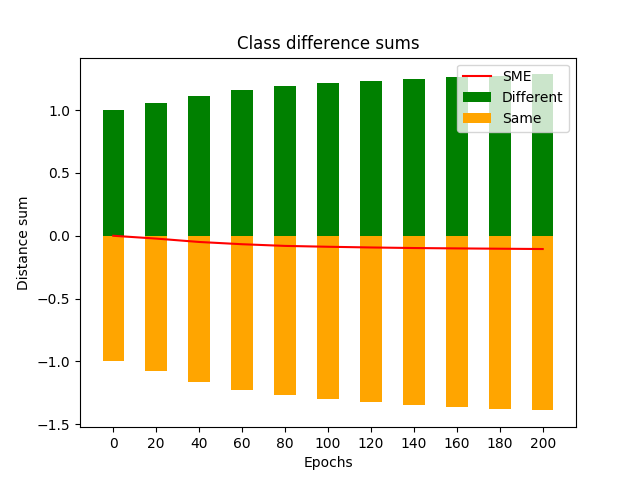
\includegraphics[width=1.\linewidth]{images/plotMethod_ClDiffSums_AIDS_E_GDL_18_23h-04m}
				\caption{SME decreasing {\footnotesize(Dataset \textit{AIDS})}}
				\label{fig:plotmethodcldiffsumsaidsegdl1823h-04mhe}
			\end{subfigure}
			\begin{subfigure}{0.45\textwidth}
				\centering
				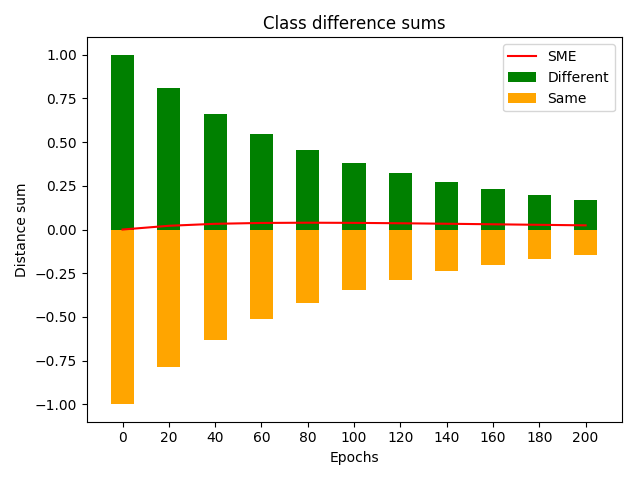
\includegraphics[width=1.\linewidth]{images/plotMethod_ClDiffSums_MSRC_9_E_GDL_22_00h-05mExp3}
				\caption{SME increasing {\footnotesize(Dataset \textit{MSRC\_9})}}
				\label{fig:plotmethodcldiffsumsmsrc9egdl2200h-05mexp3}
			\end{subfigure}
			\caption{SME error examples}
			\label{fig:SMEExamples}
		\end{figure}
	
		The two examples visualize a decreasing and thereby improving SME (\ref{fig:plotmethodcldiffsumsaidsegdl1823h-04mhe})
		and an increasing and thereby degenerating SME (\ref{fig:plotmethodcldiffsumsmsrc9egdl2200h-05mexp3}).
		Notice how the SME is decreasing, but the sum of the same cluster distances is increasing.
		Nevertheless, the decreasing SME states, that the different cluster distances are increasing faster.
		Similarly the SME is increasing, but the sum of the different cluster distances is decreasing, all be it slower than the decreasing of the same cluster distances.		

		\paragraph{Global, batch-wise and local interpretation}
		It is crucial to note, that the update rule (section \ref{subsec:EWL}) adjust the edge weights in the WLLT based on a \textit{local} evaluation of the edge weights at the time of the update.
		That is, the edge weight changes are defined using two graph samples each.
		Let us call the SME computed right after the definition of the edge weight adjustment for an individual pair of graphs in the batch the local SME.
		This local SME decreases compared to right before the definition of the edge weight adjustment every time, since the update rule is designed to do so.
		However, as described in section \ref{subsec:WLLT_ew_init}, the edge weight changes originating from comparing one pair of graphs may be changed (averaged) and are only applied after each epoch.
		Computing the SME at this point we call computing the batch-wise SME.
		It is no longer guaranteed that the SME decreases for all (hyper-)parameter settings.
		That is because changing one edge weight in the WLLT may influences the distance between several graphs, both from the same and from different classes.
		The same holds true for the global SME, which we defined first. 
		The first and most direct indicator for success of the l-WWLLT method is, to reduce this global SME.
		
		As mentioned before, we make use of additional evaluation methods.
		For example the classification accuracy using the l-WWLLT-kernel (section \ref{subsec:lWWLLTkernel}) in a support vector machine (section \ref{subsec:method_svm}), 
		or by measuring the quality of the given clusters of graph classes with respect to the similarity measure (section \ref{subsec:method_cl_eval}).
		Notice how these three evaluation methods measure different aspects of the defined similarity measure.
		After presenting these two other evaluation methods, the reasoning behind this evaluation strategy are summarized in section \ref{subsec:method_eval_strategy}.
		
	\subsubsection{Support Vector Machine} \label{subsec:method_svm}
	
		One of the easiest way to compare the performance of this learner to other methods with the similar goal to define a graph similarity measure, is to use a C-Support Vector machine (SVM)~\cite{1992_Boser_CONF, 2003_Hsu_CONF}.		
		SVMs try to define a model, which predicts target values (i.e. class labels) of features of given test data.		
		In essence, they map feature vectors with known target values (training data) into a higher (maybe infinite) dimensional space and find a linear separating hyperplane (or support vectors) with the maximal margin in this higher dimensional space.
		This hyperplane is then used for further classification decision on the test data~\cite{1992_Boser_CONF}. 
		Many researchers measure their implementations in the mean classification accuracy (and standard deviations) of a computed kernel in a $10$-fold cross validation SVM (for example \cite{2016_Kriege_NIPS, 2019_Schulz_CONF, 2011_Shervashidze_JMLR, 2020_Siglidis_CONF}) (repeated 10 times with random folds).
		That is, to partition the graph dataset in a training and evaluation set, and evaluate the performance of the computed support vectors on the training set.
		For better comparability, we use this method as well.
		
		To use a suitable SVM, the computed distance matrix is transformed into a kernel matrix using the definition of the Tree-sliced Wasserstein kernel (section \ref{subsec:lWWLLTkernel}).
		This is the main motivation to keep the edge weights positive, because this implies a positive definite kernel~\cite{2019_Le_NIPS}.
		It is recommended to scale the kernel linearly to the interval $[0,1]$.
		This scaling may reduce dominating effects of attributes with greater numeric range over those with smaller ones and it may avoid numerical difficulties during the calculation~\cite{2003_Hsu_CONF}.
		However using only non-negative distances, the kernel definition using the exponential function, and having distances of value zero on the diagonal of the distance matrix already lead to properly scaled values.
	
	\subsubsection{Cluster Evaluations} \label{subsec:method_cl_eval}
	
		In order to evaluate the already present clustering, when using the similarity measure induced by some (learned) edge weights $w$, we use the scores presented in section \ref{subsec:def_cl_scores}.
		Given the distance matrix of all graph classes according to the defined l-WWLLT-distance, no further parameters are required.
		To summarize, we use the Silhouette coefficient $S_{\text{SC}}$ to evaluate the tightness and separation of the cluster.
		An increasing Silhouette coefficient (possibly approximating $1.0$) is desirable in this application.
		We use the Davies-Bouldin score $S_{\text{DB}}$ to evaluate the similarity between the clusters.
		A decreasing Davies-Bouldin score is desirable in this application.
		We use the Calinski-Harabasz score $S_{\text{CH}}$ to evaluate the cluster dispersion.
		An increasing Calinski-Harabasz score is desirable in this application.
		
		Besides these scores, we track a multitude of other values with respect to the clustering.
		For example the maximum, minimum and mean distance between all samples the same and different classes, for all classes.
		We may refer to the distance between samples of the same class as intra-distance and to to the distance between samples of the different class as inter-distance.
		Notice that not all of these measurements have a fixed desired trajectory.
		Key indicators for an improved clustering are increasing minimum inter-distance, decreasing maximum intra-distance.
		
		As a visualization of the clustering a T-distributed Stochastic Neighbor Embedding (t-SNE)~\cite{2008_Maaten_CONF} was used\footnote{More specifically the default implementation from the package \texttt{sklearn.manifold.TSNE} on \url{https://scikit-learn.org/stable/modules/generated/sklearn.manifold.TSNE.html}.}. 
		These embeddings are able to visualize high-dimensional data by considering data point similarities as (low-dimensional) joint probabilities.
		They then try to minimize the Kullback-Leibler divergence between these.
		Note that the visualizations are not deterministic and can be visualized differently in multiple computations.
						
	\subsubsection{Method Evaluation Strategy} \label{subsec:method_eval_strategy}
	
		Measurements like the mentioned statistics of all computed distances or visualizations of the edge weights in the WLLT, the distance matrix, and the WLLT itself were used to guide the implementation and the understanding of the method.
		The experiments with the l-WWLLT method, and thus its success were guided by considering the SME, the accuracy of the implied kernel, and the implied scores of the graph clustering.		
		It is not mandatory for these three evaluations to align in their assessment. %LaterTODO: Find theoretical ideas for this
		However we assume, that if a distance matrix, reflects a clearer separation between the samples of different classes, also relates to a better accuracy of the SVM, since the optimal separating hyperplane (or support vectors) should be less faulty.
		This may be true for the other way as well. 
		Although a clear cluster separation does not improve all cluster scores equally.
			
		It is important to keep in mind, that in the training process and our experiments, the clustering is given by the dataset and not computed by the learner itself.
		We only measure that the graph structures, represented in the graph representations relates to the given graph classifications.
		This also means, that if the classifications do not relate to the WL-labels (unfolding trees), there may be little chance, that the computed weights in the WLLT can reflect the classifications at all.		
	
	\subsubsection{Comparison to Other Methods} \label{subsec:comparison_to_other_methods}
					
		After this explanation of the l-WWLLT method, we come back to the related work mentioned in section \ref{subsec:related_work} and compare this approach to similar ones.

		The researched method is similar to the WL-OA Kernel (see section \ref{subsec:def_WLOA}) but differs in an important aspect.
		While the WL-OA only considers the equal subset of WL-labelings between two graphs, our approach considers the complete comparison of all labels, and especially the differences.
		Our approach emphasizes the differences, since similarities between equal feature vectors of two graphs are reduced when computing their $L_1$-norm.
		The between different feature vectors remain when computing the $L_1$-norm.
		In other words, the WL-OA focuses on the paths of the WLLT from the root to the lowest common ancestors (WL-labels) which both graphs have in common~\cite{2016_Kriege_NIPS}.		
		Our method focuses on the part of the WLLT from the lowest common ancestor to the leaves, but considers both paths as well.
		This may seem more intuitive for the task of defining a dis-similarity measure, since all dis-similarities with respect to the WL-label representation are considered.
		Note, that unlike \citeauthor{2016_Kriege_NIPS} when proposing the WL-OA, we formulate the l-WWLLT with respect to categorical vertex labels only.
				
		As mentioned above, the Wasserstein distance depends greatly on its ground metric $d$.
		In different formulas for different Wasserstein distances given in section \ref{subsec:def_WassDist}, the ground metric is used either directly, to define the cost matrix or to define the used edge weights.						
		Using a tree metric as ground distance, allows us to use the efficient close formula definition presented in equation \ref{eq:TreeWassDist} in section \ref{subsec:def_WassDist}.
		\citeauthor{2019_Togninalli_NIPS} used the Wasserstein distance on a histogram like representation of graphs too~\cite{2019_Togninalli_NIPS}.
		But as ground metric they used the normalized Hamming distance (for categorical vertex features) or the Euclidean distance (for continuous vertex features).
		Therefore a key difference between their approach and the one presented in this thesis, is to define and alter the ground distance as a tree metric instead.		
		If the learning process can improve the overall performance of the similarity measure based on the tree metric, one may relate this performance to the performance when using the normalized Hamming distance or the Euclidean distance again.
		
		The graph representations used in the NoG Kernel by \citeauthor{2019_Schulz_CONF} only consider quantities of vertex and edge labels.
		Using a uniform edge weight initialization for the WLLT, this quantitative approach is included in the representation of the graph representation in the l-WWLLT (for the zeroth layer of the WLLT).
		One may argue, that the second layer in the WLLT holds similar information as the edge label count in the NoG.
		However we did not consider original edge labels.
		By including more layers, than just the zeroth, the l-WWLLT method includes structural information (on the neighborhoods and thus edges).
		Which differs from the NoG Kernel since it ignores structural information~\cite{2019_Schulz_CONF}.
		Note however, that depending on the dataset, the original vertex (and edge) labels themselves can contain structural information as well.
		For example in graph modeling molecular structures often include information on the used atoms in the vertex labels.
		Often, the definition of an atom relates to possible structural properties as well.
		